\chapter{Internet of Things: Technologies and Architectures}
\label{ch:iot_tech_arch}
\lhead{Chapter 2. Internet of things: Technologies and Architectures}

The \textit{Internet of things}, basically, refers to a ecosystem of interconnected physical objects that are accessible through the Internet. 
In 1998, the term ``Internet of Things" was first used in a presentation of Kevin Ashton when presenting his work in The Auto-ID Labs~\footnote{https://autoidlabs.org/}. 
Since then, this paradigm has tremendously gained attention in the scenarios of modern embedded technology, communication technology and information technology.

The vision of the IoT has been built up from different perspectives that focus on the integration of physical world with the virtual world.
This integration is being created by enabling physical objects to perceive their surrounding environment, to connect and exchange data among each other and to communicate with people.
As a result, people will be able to monitor and interact with the physical environment remotely from the computer-based systems.
On the other hand, physical objects will be able to derive an understanding of their context, to cooperate with each other, to adaptively interact to changes of their context and thus intelligently assist people.

IoT requires the integration of several technologies.
Embedded technology enables sensors and actuators to be quipped on physical objects; thus they are able to perceive their context and react adaptively to the context.
Communication technology provides networking capabilities; hence, IoT objects can communicate with each other to exchange data an context.
Internet access and user interfaces allows interaction with or provides assistance to people from anywhere and at anytime.

%====================================================================
\section{History of Internet of Things}
\label{sec:history_of_iot}
%====================================================================
The IoT is being built up by researchers, business alliances and standardisation bodies from many domains and different perspectives.
\cite{Atzori:2010} summarised that IoT would result from the convergence of three main visions: \textit{Thing-oriented vision}, \textit{Internet-oriented vision} and \textit{Semantic-oriented vision}.

%[1999]  
The very first vision of the IoT was derived from the Thing-oriented perspective.
The term ``Internet of Things" was first used in the Auto-ID lab's presentation that introduced Radio-Frequency Identification(RFID) technology. 
An RFID system is composed of RFID readers and RFID tags.
A tags has a unique identifier and is attached in a physical object.
The readers listen to the radio signal from tags to identify the appearance of physical objects in the surrounding area. 
Such RFID systems would allow physical objects to be mapped into the virtual world using RFID readers and RFID tags.
In this early stage, ``Things" simply referred to RFID tags and the IoT was a system of physical objects that were traceable via RFIDs. 
The Unique/Universal/Ubiquitous Identifier(uID)~\citep{Sakamura:2006} and the Electronic Product Code(EPC)~\citep{Armenio:2007} were the following projects that supported the worldwide use of the RFID technology.
These projects aimed to create a global standard for RFIDs that would enable the global identification for physical objects.

%[2005]
It was argued that the IoT would be built up by combing RFID technology and sensing technology~\citep{ITU:2005}.
The RFID tags could respond to the location, label and status of the tagged physical objects.
Sensors could be embedded in the physical objects to provide information about the environment surrounding the objects. 
The integration of the two technologies would enable the fuller understanding on the context of the physical objects.
Wireless sensors and RFID tags attached on moving objects would provide better status of the objects, i.e, their location and temperature, movements, etc.
The IoT vision became wider vision than the idea of a global system of RFID tagged objects, thing's intelligence was considered~\citep{Sterling:2005}. 

%[2006-2009]
According to~\cite{Presser:2009}, the IoT could be more than just a global EPC system of RFID tagged objects.
Devices, networks, services would be soon also viewed as components of the IoT.
However, RFID technology would still be the forefront of the enabling technologies of the IoT.
Together with RFID, the atomic technologies of the IoT would be Near Field Communication(NFC), Wireless Sensor and Actuator Networks(SWAN).
Wireless Identification and Sensing Platforms(WISP) was the project that aimed to create IoT platform based on these technologies~\citep{Buettner:2008}.

%[2014]
More recently, the focus on ``Things" has gone beyond the RFIDs, and the intelligence of IoT ``Things" has been the recent interest~\citep{Sundmaeker:2010}.
The ``Things" mean the ~\textit{Smart Items} which are not only equipped with usual sensors, actuators, wireless communication and elaboration capabilities, but also with new smart and adaptive potentials.
Autonomous and proactive behaviours, context awareness, collaborative communications are just some of these now potentials~\citep{Atzori:2014}.

%[internet-oriented 2005 - 2010]
According to~\cite{Atzori:2010}, the IoT vision that everything would be connected was derived from the \textit{Internet-oriented} perspective.
In 2005, the ITU Internet Reports phrased the IoT vision as ``from anytime, anyplace connectivity for anyone, we will now have connectivity for anything"~\citep{ITU:2005}.

The researches on the Internet-oriented vision attempted to extend the ``Internet of computers" to the ``Internet for everyday objects"~\citep{Mattern:2010}.
For bringing the Internet into a physical infrastructure, the Internet $\emptyset$~\citep{Gershenfeld:2006} simplified the Internet Protocol(IP) to adapt to any object.
Internet Protocol for Smart Objects(IPSO)~\citep{Dunkels:2008} proposed 6LoWPAN protocol for the connectivity on the devices that have limited processing capabilities.
IPv6 could provide larger IP space for the huge number of physical objects and 6LoWPAN allowed IPv6 packets to be transmit over low power wireless IEEE 802.15.4 links.

From the Internet-oriented perspective, the IoT would be seen as an integrated part of the ``Future Internet", people and thing would be connected ``Anytime, Anyplace, with Anything and Anyone, ideally using Any path/network and Any service"~\citep{Sundmaeker:2010}.
In this context, ``thing" could be a real/physical entity or digital/virtual entity.
The IoT could be an integrated information network of physical and virtual ``thing" that have identities, physical attributes and virtual personalities.  
Research on SOA(service oriented architecture), Web started to pay attention the adoptions for physical ``things" thus enabling such integration~\citep{De:2011, De:2012,Guinard:2009}. 
The idea ''sensing as service" was one of the efforts for enabling the accesses of sensory data through standard service technologies~\citep{Perera:2014a}. 
The ``Web of things" was created based on the idea that a ``things" could form a new Web, and Web standards could be reuse to connect and integrate into the Web of physical things.

Also, it was argued that the IoT only makes its value when the data of the physical world could be collected, analysed and transformed into useful knowledge~\citep{Vermesan:2011}.
The volume and variety of ``Things" would poses challenges of how to store, interconnect, search and organise the information generated by the IoT. 
The ideas that the semantic technologies would play the key role in solving these challenges formed the Semantic-oriented vision of the IoT~\citep{Atzori:2014,Barnaghi:2012}.
IoT devices and IoT data can be efficiently discoverable and searchable by providing them semantic description~\citep{Ioan:2009, Chun:2015,Serena:2017}. 
Adding meaningful description for IoT data would also allow the data to be understandable to machines and software agents, thus facilitating the automated interaction among IoT devices and interoperability among existing IoT platforms~\citep{IERC:2015, Ganzha:2017}. 
Moreover, with semantic annotated data, IoT systems could better understand the context, thus creating smarter services~\citep{Perera:2014a}. 






\section{IoT Technologies}



\subsection{Identification}

Identification is crucial for the IoT to name and match
services with their demand. Many identification methods are
available for the IoT such as electronic product codes (EPC) and
ubiquitous codes (uCode) [21]. Furthermore, addressing the
IoT objects is critical to differentiate between object ID and its
address. Object ID refers to its name such as “T1” for a particular
temperature sensor and object’s address refers to its address
within a communications network. In addition, addressing
methods of IoT objects include IPv6 and IPv4. 6LoWPAN [22],
[23] provides a compression mechanism over IPv6 headers
that makes IPv6 addressing appropriate for low power wireless
networks. Distinguishing between object’s identification and
address is imperative since identification methods are not globally
unique, so addressing assists to uniquely identify objects.
In addition, objects within the network might use public IPs
and not private ones. Identification methods are used to provide
a clear identity for each object within the network.

- URIs 

Device/Objects/Things Identification, Addressing, and
Discovery: Scalable addressing and identification mechanisms
are required for IoT because of the continuous increase in the
number of connected devices. Moreover, the design of such
scalable mechanisms is being challenged by the heterogeneity
of devices, which are configured with the IP as well as
a non-IP addressing format. Therefore, the primary goal of
research efforts in this area is to address the challenges of
device identification and addressing by designing lightweight
protocols and schemes that support flexible address allocation,
address collision or duplicate address detection (for security),
address recycling, address translation, and auto-configuration
of addresses by devices. Such addressing protocols are necessary
for scalable and seamless ubiquitous connectivity in the
IoT ecosystem.

Furthermore, as indicated in ISO 15459, multiple
established name issuing authorities
exist and it is important that the Internet of
Things recognises their legitimate but nonexclusive
involvement in the construction of
unique identifiers for things and in helping to
manage delegation of uniqueness of the identifiers
created by their members, each of
whom is thereby granted the autonomy to
create unique identifiers within their own
namespace; it should also be possible for
anyone to use Uniform Resource Identifiers
(URI) as unique identifiers for things.
It is important to understand that identifiers
can refer to names and addresses, but since
there can be multiple addresses of information
and services related to an individual
thing, it is probably more helpful to ensure
that each thing is given a unique name and to
use lookup mechanisms and referral services
to obtain addresses of information and services,
including those provided authoritatively
by the thing's creator and those contributed
by others who have interacted with
the thing at some time in its life. In the case
of the existence of multiple identifiers for a
single object due to different reasons a
scheme for ID data translation and dynamic
compatibility/interoperability check is necessary


Depending on various technologies for the implementation,
the definition of the IoT varies. However, the fundamental
of IoT implies that objects in an IoT can be identified
uniquely in the virtual representations. Within an IoT, all
things are able to exchange data and if needed, process data
according to predefined schemes.


\subsection{Sensing}

The IoT sensing means gathering data from related objects
within the network and sending it back to a data warehouse,
database, or cloud. The collected data is analyzed to take speci-
fic actions based on required services. The IoT sensors can be
smart sensors, actuators or wearable sensing devices. For example,
companies like Wemo, revolv and SmartThings offer smart
hubs and mobile applications that enable people to monitor
and control thousands of smart devices and appliances inside
buildings using their smartphones [24]–[26].
Single Board Computers (SBCs) integrated with sensors and
built-in TCP/IP and security functionalities are typically used
to realize IoT products (e.g., Arduino Yun, Raspberry PI, BeagleBone
Black, etc.). Such devices typically connect to a central
management portal to provide the required data by customers.


\subsection{Communication}

The IoT communication technologies connect heterogeneous
objects together to deliver specific smart services. Typically, the
IoT nodes should operate using low power in the presence of
lossy and noisy communication links. Examples of communication
protocols used for the IoT are WiFi, Bluetooth, IEEE
802.15.4, Z-wave, and LTE-Advanced. Some specific communication
technologies are also in use like RFID, Near Field Communication
(NFC) and ultra-wide bandwidth (UWB). RFID is
the first technology used to realize the M2M concept (RFID
tag and reader). The RFID tag represents a simple chip or label
attached to provide object’s identity. The RFID reader transmits
a query signal to the tag and receives reflected signal from the
tag, which in turn is passed to the database. The database connects
to a processing center to identify objects based on the re-
flected signals within a (10 cm to 200 m) range [27]. RFID tags
can be active, passive or semi-passive/active. Active tags are
powered by battery while passive ones do not need battery.
Semi-passive/active tags use board power when needed.
The NFC protocol works at high frequency band at 13.56 MHz
and supports data rate up to 424 kbps. The applicable range is
up to 10 cm where communication between active readers and
passive tags or two active readers can occur [28]. The UWB communication
technology is designed to support communications
within a low range coverage area using low energy and high
bandwidth whose applications to connect sensors have been
increased recently [29].
Another communication technology is WiFi that uses radio
waves to exchange data amongst things within 100 m range
[30]. WiFi allows smart devices to communicate and exchange
information without using a router in some ad hoc configurations.
Bluetooth presents a communication technology that is
used to exchange data between devices over short distances using
short-wavelength radio to minimize power consumption [31].
Recently, the Bluetooth special interest group (SIG) produced
Bluetooth 4.1 that provides Bluetooth Low Energy as well as
high-speed and IP connectivity to support IoT [32]. The IEEE
802.15.4 standard specifies both a physical layer and a medium
access control for low power wireless networks targeting reliable
and scalable communications [33].

LTE (Long-Term Evolution) is originally a standard wireless
communication for high-speed data transfer between mobile
phones based on GSM/UMTS network technologies [34]. It
can cover fast-travelling devices and provide multicasting and
broadcasting services. LTE-A (LTE Advanced) [35] is an improved
version of LTE including bandwidth extension which
supports up to 100 MHz, downlink and uplink spatial multiplexing,
extended coverage, higher throughput and lower latencies

\subsection{Computation}

Processing units (e.g., microcontrollers, microprocessors,
SOCs, FPGAs) and software applications represent the “brain”
and the computational ability of the IoT. Various hardware platforms
were developed to run IoT applications such as Arduino,
UDOO, FriendlyARM, Intel Galileo, Raspberry PI, Gadgeteer,
BeagleBone, Cubieboard, Z1, WiSense, Mulle, and T-Mote Sky.
Furthermore, many software platforms are utilized to provide
IoT functionalities. Among these platforms, Operating Systems
are vital since they run for the whole activation time of a
device. There are several Real-Time Operating Systems (RTOS)
that are good candidates for the development of RTOS-based IoT
applications. For instance, the Contiki RTOS has been used
widely in IoT scenarios. Contiki has a simulator called Cooja
which allows researcher and developers to simulate and emulate
IoT and wireless sensor network (WSN) applications [36].
TinyOS [37], LiteOS [38] and Riot OS [39] also offer light
weight OS designed for IoT environments. Moreover, some
auto industry leaders with Google established the Open Auto
Alliance (OAA) and are planning to bring new features to the
Android platform to accelerate the adoption of the Internet of
Vehicles (IoV) paradigm [40]. Some features of these operating
systems are compared in Table I.
Cloud Platforms form another important computational part
of the IoT. These platforms provide facilities for smart objects
to send their data to the cloud, for big data to be processed
in real-time, and eventually for end-users to benefit from the
knowledge extracted from the collected big data. There are a
lot of free and commercial cloud platforms and frameworks
available to host IoT services. Some of these services are
introduced in Section VII-B.

\subsection{Services}

Overall, IoT services can be categorized under four classes
[41], [42]: Identity-related Services, Information Aggregation
TABLE II
BUILDING BLOCKS AND TECHNOLOGIES OF THE IOT
Services, Collaborative-Aware Services and Ubiquitous Services.
Identity-related services are the most basic and important
services that are used in other types of services. Every
application that needs to bring real world objects to the virtual
world has to identify those objects. Information Aggregation
Services collect and summarize raw sensory measurements
that need to be processed and reported to the IoT application.
Collaborative-Aware Services act on top of Information Aggregation
Services and use the obtained data to make decision and
react accordingly. Ubiquitous Services, however, aim to provide
Collaborative-Aware Services anytime they are needed to anyone
who needs them anywhere. With this categorization, we review
some applications of the IoT in the following paragraphs.
The ultimate goal of all IoT applications is to reach the level of
ubiquitous services. However, this end is not achievable easily
since there are a lot of difficulties and challenges that have to be
addressed. Most of the existing applications provide identityrelated,
information aggregation, and collaborative-aware services.
Smart healthcare and smart grids fall into the information
aggregation category and smart home, smart buildings, intelligent
transportation systems (ITS), and industrial automation
are closer to the collaborative-aware category.

\subsection{Semantic}
Semantic in the IoT refers to the ability to extract knowledge
smartly by different machines to provide the required services.
Knowledge extraction includes discovering and using resources
and modeling information. Also, it includes recognizing and
analyzing data to make sense of the right decision to provide
the exact service [62]. Thus, semantic represents the brain of the
IoT by sending demands to the right resource. This requirement
is supported by Semantic Web technologies such as the Resource
Description Framework (RDF) and the Web Ontology
Language (OWL). In 2011, the World Wide Web consortium
(W3C) adopted the Efficient XML Interchange (EXI) format as
a recommendation [63].
EXI is important in the context of the IoT because it is designed
to optimize XML applications for resource-constrained
environments. Furthermore, it reduces bandwidth needs without
affecting related resources such as battery life, code size,
energy consumed for processing, and memory size. EXI converts
XML messages to binary to reduce the needed bandwidth
and minimize the required storage size.
Remarks: In this section, the main components of the IoT
were identified along with their related standards, technologies
and realizations. The variety of standards and technologies in
these elements and the way they should interoperate is a main
challenge that can impede the development of IoT applications.
The heterogeneity of the IoT elements needs a thorough solution
to make ubiquitous IoT services a reality. Section VIII
addresses this problem by proposing an architectural model that
alleviates the interoperability issues caused by the diversity of
protocols and technologies utilized in the context of the IoT.

\section{IoT Architectures}
ummarizing, although huge efforts have been made within the IERC
community for the design and development of IoT technologies, the con-
tinuously changing IoT landscape and the introduction of new requirements
and technologies creates new challenges or raise the need to revisit existing
well-acknowledged solutions. Thus, below is a list of the main open research
challenges for the future of IoT:
• IoT architectures considering the requirements of distributed intelli-
gence at the edge, cognition, artificial intelligence, context awareness,
tactile applications, heterogeneous devices, end-to-end security, privacy,
trust, safety and reliability.
• IoT systems architectures integrated with network architecture forming
a knowledge-centric network for IoT.
• Intelligence and context awareness at the IoT edge, using advanced
distributed predictive analytics.
• IoT applications that anticipate human and machine behaviours for
social support.
• Tactile Internet of Things applications and supportive technologies.
• Augmented reality and virtual reality IoT applications.
• Autonomics in IoT towards the Internet of Autonomous Things.
• Inclusion of robotics in the IoT towards the Internet of Robotic Things.
Artificial intelligence and machine learning mechanisms for automating
IoT processes.
• Distributed IoT systems using securely interconnected and synchronized
mobile edge IoT clouds.
• Stronger distributed and end-to-end holistic security solutions for IoT,
preventing the exploitation of IoT devices for launching cyber-attacks,
i.e., remotely controlling IoT devices for launching Distributed Denial
of Service (DDoS) attacks.
• Stronger privacy solutions, considering the requirements of the new
General Data Protection Regulation (GDPR) [80] for protecting the
users’ personal data from unauthorized access, employing protective
measures (such as Privacy Enhancing Technologies – PETs) as closer
to the user as possible.
• Cross-layer optimization of networking, analytics, security, communi-
cation and intelligence.
• IoT-specific heterogeneous networking technologies that consider the
diverse requirements of IoT applications, mobile IoT devices, delay
tolerant networks, energy consumption, bidirectional communication
interfaces that dynamically change characteristics to adapt to application
needs, dynamic spectrum access for wireless devices, and multi-radio
IoT devices.
• Adaptation of software defined radio and software defined networking
technologies in the IoT.


\subsection{Edge Computing}

Three typical edge computing solution:

- cloudet 

- Mobile edge computing

- Fog computing

Obviously, the IoT could benefit from cloud infrastructures~\citep{Botta:2016} in providing computational resource for processing IoT data.
The cloud computing has been a mature technology and has been considered as an unlimited capabilities storage and processing power.
The IoT also has been integrated with the cloud computing that introducing the \textit{``Cloud of Things"}~\citep{Jiehan:2013} or the ~\textit{``IoT Cloud"}~\citep{Truong:2015}.
These cloud-based systems allow IoT data to be uploaded into cloud, and after being processed, the requesting results are sent back to the IoT devices or IoT applications.

Although cloud infrastructures have been efficient for processing IoT data as computational resources on the cloud outclasses that of IoT devices at the edge, cloud computing solution could not completely solve the scalability issue in the IoT.
The end devices in the IoT are not only data consumers as in cloud computing paradigm but data producers.
Therefore, the common approaches of directly connecting IoT devices and pushing IoT data to the cloud may have several disadvantages~\citep{Zhang:2015}.
The increasing of the number of the IoT devices means the quantity of produced IoT data is raising quickly.
Most of the data can be discarded immediately after being processed.
Hence, in these centralised systems, the bandwidth would be overwhelming and might be wasted.
Furthermore, pushing data into cloud will dominate upstream network traffic, meanwhile, broadband networks have more downstream bandwidth than upstream bandwidth.
Moreover, some IoT applications might require very quick response time, unfortunately, cloud-based solution may lead these applications to be less operable due to unexpected network latencies.
In additional, IoT data might contain sensitive information from the sensors that are implanted surrounding us.
Cloud-based systems create more privacy and security concerns as centralised storages are out of users' control.

Edge computing~\citep{Salman:2015} has been the recently decentralised computing paradigm to address these issues.
\cite{WShi:2016} explained that ``edge computing refers to the enabling technologies allowing computation to be performed at the edge of the network,
on downstream data on behalf of cloud services and upstream data on behalf of IoT services".
\cite{WShi:2016} also defined the ``edge" as ``any computing and network resources along the path between data sources and cloud data centres".
Thus, the edge can be the smartphones as they are placed between sensors and cloud or the edge can be the gateway devices that connect smart devices and data centres.

The edge computing has been emergent and benefit for the IoT~\citep{Yu:2018}. 
There have been several early results that demonstrated the benefit of applying edge computing. 
Face recognition application could run 4 times faster by moving computation from cloud to edge~\citep{Yi:2015}.
Using cloudets for offloading computing tasks did not only reduce the response time for wearable cognitive assistant but also save 30$\%$ to 40$\%$ energy consumption~\citep{Ha:2014}. 
However, computing nodes often have less computational resource and networking capability. 
This poses a challenge for the computing tasks to be physically moved to the edge nodes.












\section{Conclusion}

IoT developments during recent years have been characterized by
attributes that can be “labelled” the 6As: Anything (any device), to be
transferred from/to Anyone (anybody), located Any place (anywhere), at
Any time (any context), using the most appropriate physical path from Any
path (any network) available between the sender and the recipient based
on performance and/or economic considerations, to provide Any service
(any business). The IoT paradigm is evolving and entire IoT ecosystems
are now built upon innervation elements known as the 6Cs: Collect (het-
erogeneity of devices of various complexities and intelligence, that enhance
the real-time collection of data generated from the connections of devices
and information), Connect (ubiquitous distributed connections of heteroge-
neous devices and information, where the connections are the foundational
component of the IoT), Cache (stored information in the distributed IoT com-
puting/processing environment), Compute (advanced processing and com-
putation of data and information), Cognize (information analytics, insights,
extractions, real-time AI processing and Create (the creation of new interac-
tions, services, experiences, business models and solutions). This is illustrated
in Figure 3.1






















\nop{

%==================================================================================================
\section{The Semantic Web technology}
\label{s:sw}
%==================================================================================================

According to World Wide Web Consortium(W3C), the Semantic Web technologies aim to ``provide a common framework that allows data to be shared and reused across application, enterprise, and community boundaries".
The Semantic Web community has developed a suite of standards and technologies to formally describe the semantics, support automated reasoning on web data.
As we mentioned in Section~\ref{ss:stiot}, such technologies developed by the Semantic Web are potentially the solutions to data integration, semantic interoperability, context awareness and knowledge transformation in the IoT.
This section introduces the core technologies of the Semantic Web that including Resource Description Framework~\citep{Lassila:1999},RDF schema~\citep{Dan:2004}, Web ontology language~\citep{Guinnes:2004} and SPARQL query language~\citep{Eric:2008}.

%===================================================
\subsection{RDF Data Model}
\label{ss:rdf}
%===================================================
A \textit{data model} is an abstraction that is used to represent the information of real world entities.
It defines how the properties and relations of the entities are represented, and the operations can be performed on the information.
Data models can be categorised as relational, tree and graph based. 

\begin{figure}[ht!]
	\centering
	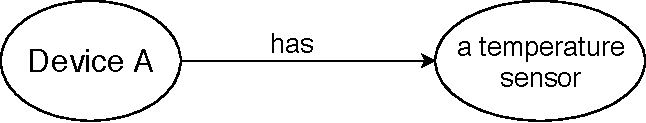
\includegraphics[scale=.65]{c2/2-2-SimpleTriple.pdf}
	\caption{A triple}
	\label{fig:2.2-simpleTriple}
\end{figure}

RDF data model is a graph-based data model. 
Its design is based on the idea that things can be represented by statements in a simple manner of triples. 
The statement is similar to a simple sentence that has subject, verb, object.
The triple is composed of three elements: a subject, a predicate and an object that represent the statement.
For example, the sentence "Device A has a temperature sensor" can be expressed as a triple as follows: ``Device A" is the subject, ``has" is the predicate and ``a temperature sensor" is the object.
The statement can be visually expressed in Figure~\ref{fig:2.2-simpleTriple}

An RDF triple is built from \textit{IRIs} (International Resource Identifiers), \textit{literals} and \textit{blank nodes} which are also called \textit{resources}~\citep{Cyganiak:2014}. 
RDF triple can be formally define as follow:
``An RDF triple is a tuple (S, P, O) $\in$ (I$\cup$B)  $\times$ I $\times$ (I$\cup$B$\cup$L), where S is the subject, P is the predicate and O  is the object and I, B and L are used to represent IRIs, blank nodes and literals respectively."

The IRI is a unique identifier that presents a thing or a concept.
For example, the IRI for representing the device A in the previous example might be ``\textit{http://insight.org/device/A}". 
The IRI ``\textit{http://insight.org/sensor/temperature}" can refer to the concept of ``temperature sensor".
Literals are used to represent value data types such as numbers, booleans or strings. 
A literal might be a simple string such as ``a temperature sensor", or with a optional language tag, ``a temperature sensor"$@$en, 
denoting the language (English), or with an IRI, ``temperature sensor"{\symbol{94}\symbol{94}}\textit{http://www.3.org/2001/XMLSchmea$\#$String}, assigning the datatype (String). 
The blank node (B-Node) is used to refer to a concept with giving it a name. 
The usage of the blank will be explained shortly in the later example.

In an RDF triple, the subject is an IRI or a blank node as it must refer to a concept. 
The object can be an IRI, a blank node or literal. 
The predicate is guaranteed to be an IRI denoting a bi-relationship between the two resources. 
Figure~\ref{fig:2.3-SimpleRDFTriple} shows the presentation of the previous example statement as an RDF triple.

\begin{figure}[ht!]
	\centering
	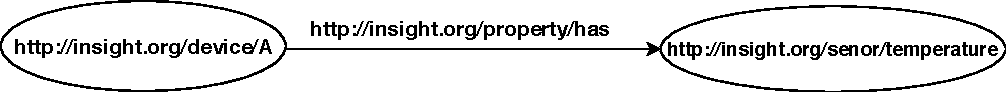
\includegraphics[scale=0.75]{c2/2-3-SimpleRDFTriple.pdf}
	\caption{An RDF Triple }
	\label{fig:2.3-SimpleRDFTriple}
\end{figure}

An RDF document is a set of RDF triples.
The RDF document can be represented as a directed graph as illustrated in Figure~\ref{fig:2.4-SimpleRDFGraph}.
The nodes represent subjects and objects, the predicates are represented by labelled edges with the direction from subjects to objects. 
Therefore, RDF documents are also called RDF graphs.

\begin{figure}[ht!]
	\centering
	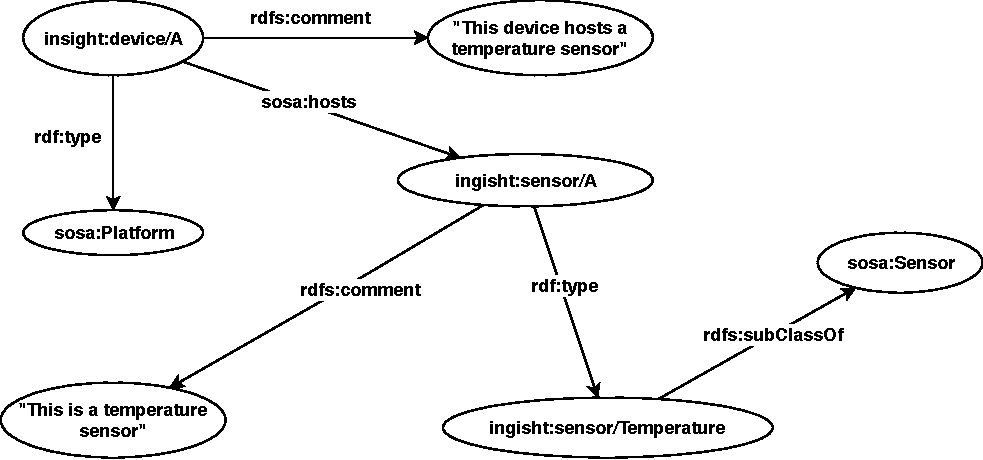
\includegraphics[scale=0.65]{c2/2-4-SimpleRDFGraph.pdf}
	\caption{RDF document describing device A as an RDF Graph.}
	\label{fig:2.4-SimpleRDFGraph}
\end{figure}

\textit{Vocabularies} are used to define concepts and their relations that related to a specific domains. 
For example, to describe people and their relationship, FOAF~\citep{Dan:2010} can be used.
SSN~\citep{Armin:2017} is another RDF vocabulary used for describing devices, sensors.
An RDF vocabulary is a collection of IRIs that used for describing schema and instance data.
The IRIs in an RDF vocabulary are often created with a common substring in the beginning which is called \textit{namespace} of an vocabulary.
For convenience, prefixes can be used to shorten the string representation of these IRIs.
Figure~\ref{fig:2.4-SimpleRDFGraph} illustrated the RDF document describing the devices A from the previous example.
RDFS vocabulary~\citep{Dan:2014}, which is used to defined and documented additional RDF vocabularies, and the SSN vocabulary are used.
For simplicity, prefixes are use the replace the namespaces and the list of prefixes and their corresponding namespace is shown in Listing~\ref{lst:prefixes}.

\vspace{5mm}
\begin{lstlisting}[language=sparql,
  				   captionpos=b,
                   label={lst:prefixes},
                   caption={Prefixes}]  
rdf  : <http://www.w3.org/1999/02/22-rdf-syntax-ns#>
rdfs : <http://www.w3.org/2000/01/rdf-schema#>
sosa : <http://www.w3.org/ns/sosa/>
geo  : <http://www.w3.org/2003/01/geo/wgs84_pos#>
insight : <http://insight.org/>
\end{lstlisting}


The flexible and expressivity of triple lead RDF data model become a great ideal to deal with the dynamic and heterogeneity of the IoT.
RDF  provides both ability to specify concept and ability to link different concepts together.
This enables heterogeneous IoT data to be update and integrated with extremely low effort.

\begin{figure}[ht!]
	\centering
	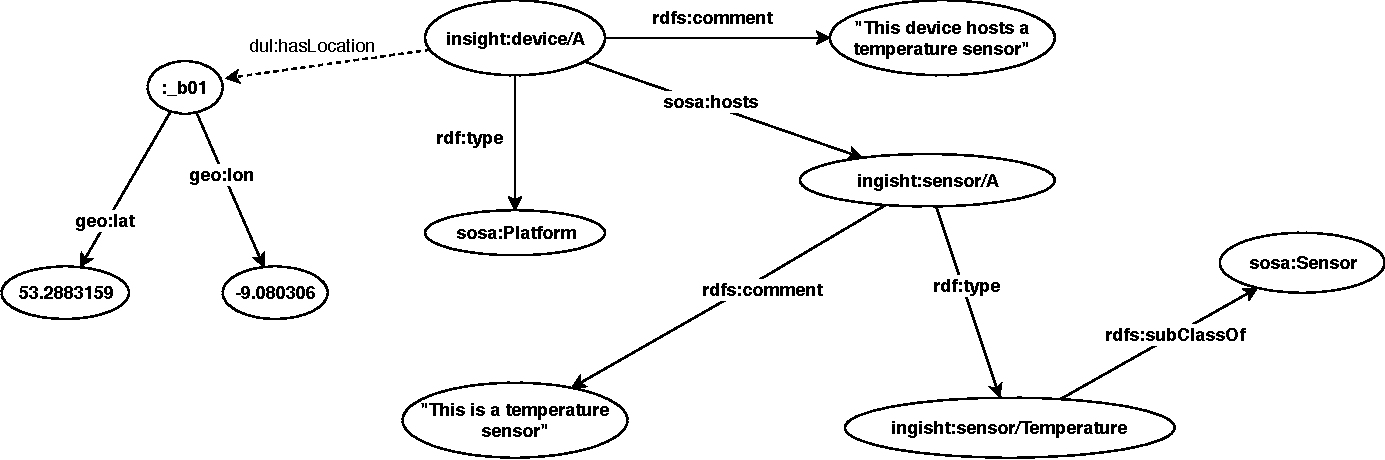
\includegraphics[scale=0.65]{c2/2-5-RDF-integration.pdf}
	\caption{Example of integration RDF graph describe device and RDF graph describing geographic coordinates}
	\label{fig:2.5-integration}
\end{figure}

As a graph data model, to represent information, RDF does not require a predefined data schema as relational databases does.
New type of information, new concept can be introduced without the need of updating data schema.
For example, to give the device A a location requires an integration of the RDF graph from Figure~\ref{fig:2.4-SimpleRDFGraph} with another RDF graph that describes the geographic coordinates.
In Figure~\ref{fig:2.5-integration}, the latitude and longitude values can be added to the RDF graph without introducing what are they.
The machine can understand via the vocabulary that is used to describe the values.
The integration is done by adding a triple to say that device A has located at a point which has the latitude, longitude values as in the figure.
This is much easier than realigning the data schema in case using common relational data model. 
In this example, the location is presented as a blank node as it does not have to be an IRI.

RDF data model allows data to be reusable and shareable.
The same vocabularies can be used in different applications, systems from different domains to describe the same thing.
For example, the vocabulary describing coordinates in a geographic application can be used to describe the location of the device.
Further more, with inferencing (see Section~\ref{ss:inference}), new relationships or concepts can be discovered from the the base relationship found in dataset.
This helps machine to determine if different vocabularies were used to describe the same concept.
In the previous example, the sensor ``\textit{insight:sensor/A}" is defined as ``\textit{a temperature sensor}" using IRI ``\textit{insight:sensor/Temperature}".
By defining ``\textit{insight:sensor/Temperature}" is the subclass of ``\textit{sosa:Sensor}", machine can understand that ``\textit{insight:sensor/A}" also refers to a sensor.
Thus, ``\textit{insight:sensor/A}" is understandable and discoverable as a sensor by another systems or applications that are using SSN vocabulary.

\textit{Linked Data} is an approach for publishing and consuming structured data on the Web using RDF data model.
The principles of Linked data include: (i) Using URIs for naming things; (ii) Using HTTP URIs to enable the look up on things; (iii) Describing the information of the URIs using RDF data; (iv) Including the links to other URIs, so that they can discover more things. 
The same principles can be applied for publishing and consuming IoT data, for example, sensor data~\citep{Patni:2010} or stream data~\citep{Sequeda:2009}.
Linked Data can make data linkable and discoverable thus becomes an efficient solution for the fragmentation issue in the IoT.
RDF data model provides a flexible way to describe things and their relationship, such as devices, observations or measurements. 
RDF vocabularies and inference allow semantics, knowledge to be shared crossing devices, systems and platforms. 
Using Linked Data principles and RDF data model could enable the semantic interoperability for the IoT in the global scale~\citep{Le-Phuoc:2018}.

%===================================================
\subsection{Inference}
\label{ss:inference}
%===================================================

As we mentioned in the previous example, the Semantic Web technologies do not only provide RDF data model to describe concepts and theirs relationships but also the ability to discover new relationships from the given dataset.
This ability is known as inference.
\textit{RDFS}(RDF schema)~\citep{Dan:2004} and \textit{OWL}(Ontology Web Language)~\citep{Guinnes:2004} are the two standards to create vocabularies that enables the inference.

RDFS is derived from RDF by adding some basic constructs to allow the inferencing on the type of things and properties of things.
RDFS is added classes and subclasses to specify different concepts and to describe if two concepts are related.
As shown in the example (see Figure~\ref{fig:2.5-integration}), the device and the sensor are differentiated by the class ``\textit{sosa:Platform}" and ``\textit{insight:sensor/Temperature}". 
The additional triple that says the type ``\textit{insight:sensor/ Temperature}" is a subclass of the type ``\textit{sosa:Sesnor}" infers that the sensor also has type ``\textit{sosa:Sesnor}".
The further additional features are property domains and ranges.
The domains of a property state that any subject that has this property is an instance of a specific class or set of classes.
The ranges of a property define the specific classes (types) that its object can be.

OWL provides more inferencing capability. 
OWL enables the ability to share not just information, but vocabulary.
For example, OWL includes ``\textit{owl:sameAs}" to state if two classes or two properties are the same.
With OWL supporting, two systems that do not use the same vocabulary to publish RDF data might be able to understand and process data the other. 

%===================================================
\subsection{SPARQL Query}
\label{ss:sparql}
%===================================================

SPARQL has been standardised as the query language query RDF data by the the World Wide Web Consortium~\citep{Eric:2008}.
To query graph-based data, SPARQL is designed as a graph-matching query language.
The graph pattern in a SPARQL query can be simple with a single triple pattern of very complex.
Given an RDF graph G and a query Q that consists of a graph pattern, the values obtained form the matching of the pattern against G are formed the answer.

A triple pattern is similar to an RDF triple in which subject, predicate, object could be a variable.
A set of triple pattern forms a basic graph pattern. 
Listing~\ref{lst:SPARQL1} is showing Q1, an example of a SPARQL SELECT query with a simple graph pattern containing a triple pattern.
The query asks for the list of the sub-systems that are hosted on the Device A.

\vspace{5mm}
\begin{lstlisting}[language=sparql,
  				   captionpos=b,
                   label={lst:SPARQL1},
                   caption={Q1 - SPARQL Query with a graph pattern}]  
PREFIX sosa    : <http://www.w3.org/ns/sosa/>
PREFIX insight : <http://ingisht.org/>

SELECT ?subSystem WHERE
{ 
  <insight:Devcie/A> sosa:hosts ?subSystem.
}    		
\end{lstlisting}


A basic graph pattern matches against a RDF graph when the variables can be replaced by values from the graph and form a subgraph of the graph.
For example, the IRI ``\textit{insight:sensor/A}" is replaced the variable ``\textit{?subSystem}" to form a subgraph of the RDF graph in Figure~\ref{fig:2.4-SimpleRDFGraph}.
This value is the answer of the query Q1 against RDF graph in Figure~\ref{fig:2.4-SimpleRDFGraph}.

A more complex may contains more than one basic graph pattern.
A resultant RDF subgraph can be further queried or joined with the results of other basic graph patterns to answer the query.
The query Q2 in Listing~\ref{lst:SPARQL2} asks for a list of subsystems on the device A that are temperature sensors.
The query contains two basic graph patterns, the first pattern asks for the subsystem on the device A and the second pattern asks if its is a temperature sensor.

\vspace{5mm}
\begin{lstlisting} [language=sparql,
  				   captionpos=b,
                   label={lst:SPARQL2},
                   caption={Q2 - SPARQL Query with multiple graph patterns}]                    
PREFIX ssn  : <http://www.w3.org/ns/ssn/>
PREFIX ex   : <http://example.org/>
PREFIX rdf  : <http://www.w3.org/1999/02/22-rdf-syntax-ns#>

SELECT ?subsystem WHERE
{ 
  <insight:Devcie/A> sosa:hosts ?subSystem.
  ?subSystem rdf:type <insight:sensor/Temperature>
}    		
\end{lstlisting}

SPARQL queries may also have additional operations including unions, optional, filter, subqueries, value aggregations, path expressions, etc.
The examples of SPARQL queries with other operations can be found in Appendix~\ref{app:A}.
Formally, a SPARQL graph pattern is a basic graph with or without these additional operations and can be summarised as following:
\begin{itemize}[noitemsep,nolistsep]
\item \textit{Group graph patterns:} A set of graph patterns delimited by braces $\{$ $\}$.
\item \textit{OPTIONAL patterns:} A graph patten identified by OPTIONAL keyword to mark this graph pattern as an optional graph pattern. 
                                  This means, the result set is returned even if the variables in the optional graph pattern are not bound.
\item \textit{UNION patterns:} Keyword UNION is used to combine graph patterns with alternative graph patterns that may match.
\item \textit{FILTER expressiond:} FILTER is used to eliminated the solution that is not match specific conditions. 
                                   The filter may be a comparison expression, logical connectives or built-in function.
\item \textit{Subqueries:} Embedded SPARQL queries that are nested inside a SPARQL query to limit the result set.
\item \textit{Property paths:} Property path is used to define the possible route through an RDF graph between two RDF nodes. 
\end{itemize}

\cite{Perez:2009} defined a SPARQL graph pattern recursively as following:
\begin{enumerate}[noitemsep,nolistsep]
\item A triple pattern is a graph pattern.
\item A graph pattern is a graph pattern.
\item If P$_{1}$, P$_{2}$ are graph pattern, then (P$_{1}$ AND P$_{2}$), (P$_{1}$ OPTIONAL P$_{2}$) and (P$_{1}$ UNION P$_{2}$) are graph patterns. 
\item If P is a graph pattern and F is a FILTER expression, then (P FILTER F) is a graph pattern.
\item If P is a graph pattern and G $\in$ ($U \cup V$), then (GRAPH G P) is a graph pattern.
\end{enumerate}

\cite{Perez:2009} also proved that for a given RDF data D, a graph pattern P, to evaluate if a mapping $\mu$ is the a result of matching 
P against D, the complexity can be summarised as follow:
\begin{itemize}[noitemsep,nolistsep]
\item The evaluation can be solved in time \textbf{O($|$P$|$.$|$D$|$)} for graph pattern expressions constructed by using only AND and FILTER operators.
\item The evaluation is \textbf{NP-complete} for graph pattern expressions constructed by using only AND, FILTER and UNION operators.
\item The evaluation is . Evaluation is \textbf{PSPACE-complete} for graph pattern expressions.
\item The evaluation(P) is in \textbf{{LOGSPACE}} for every graph pattern expression P.
\end{itemize}

In practice, SPARQL processors often join the triples that match triple patterns in a basic graph pattern. 
A basic graph pattern can be formed as a directed graph and it has different shapes(see. Figure~\ref{fig:2.6-bgp}). 
The shape of the graph pattern also defines the complexity of the matching, because, each shape requires a specific joining plan~\citep{Hartig:2014}.
The shapes of a basic graph pattern are: 
\begin{itemize}[noitemsep,nolistsep]
\item \textit{Chain} shape contains of object-subject joins as triple patterns are connected like a chain.
\item \textit{Star} shape contains subject-subject joins as the join variables are the subjects of the triple patterns.
\item \textit{Snowflake} shape is a combination of star shape and chain shape.
\end{itemize}

\begin{figure}[ht!]
	\centering
	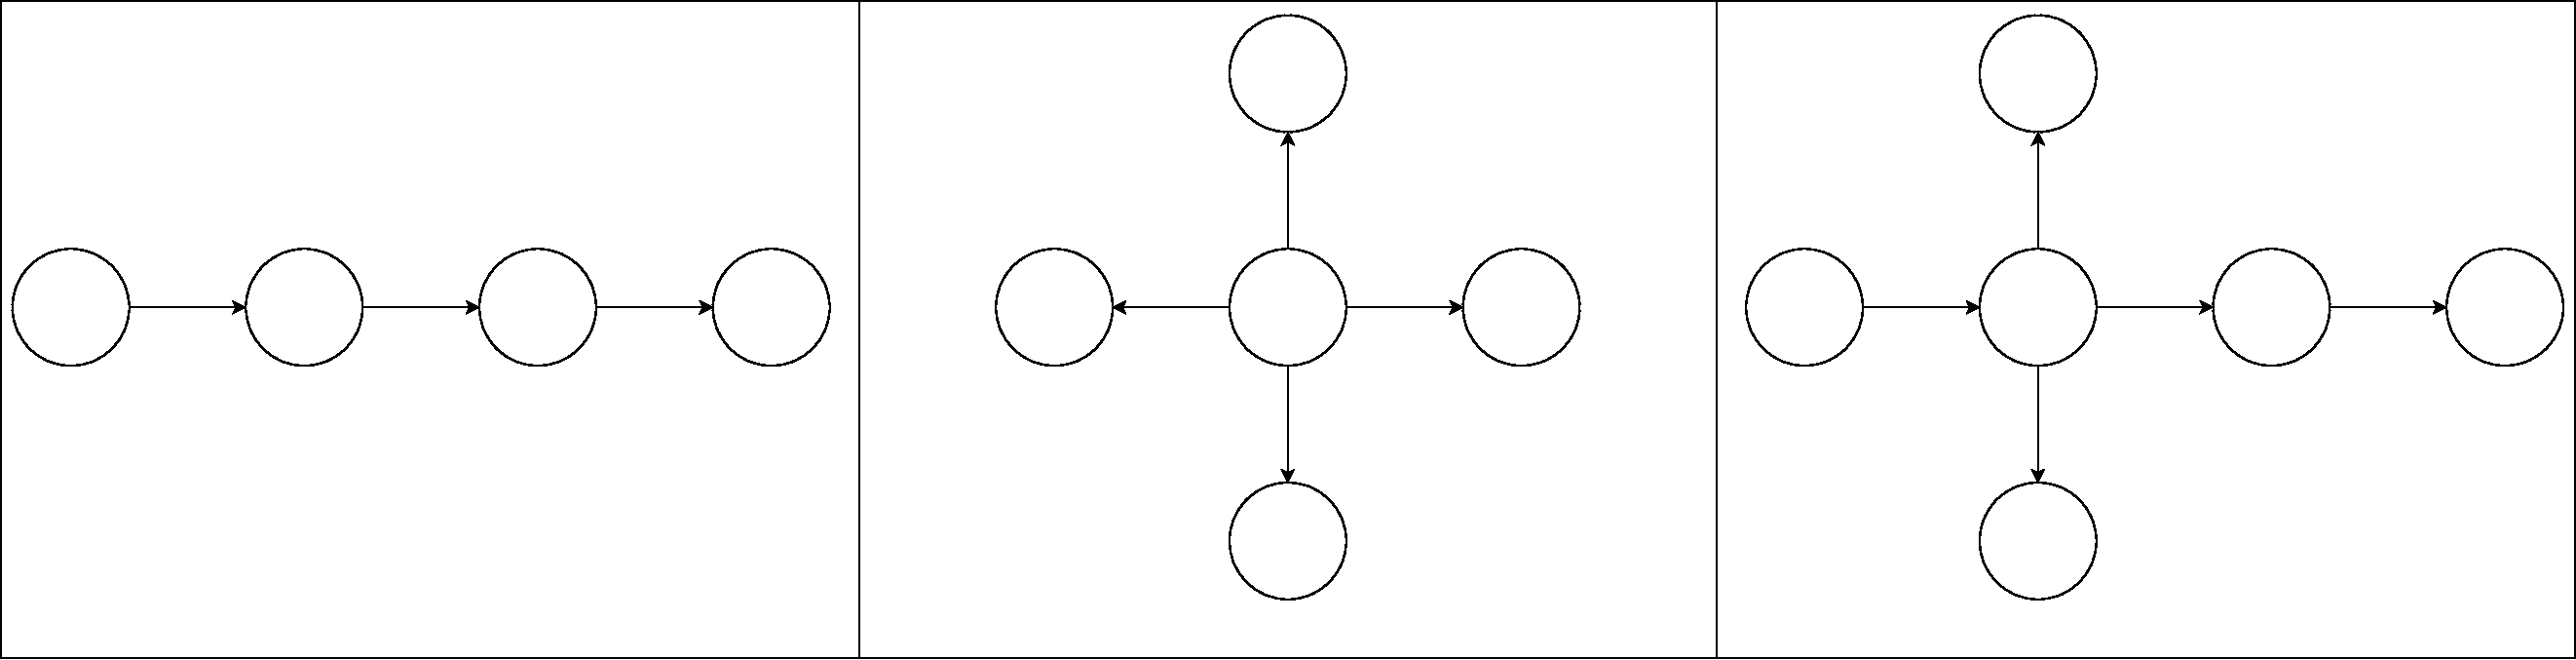
\includegraphics[scale=0.25]{c2/2-6-BGP-shape.pdf}
	\caption{Shape of basic graph pattern: chain, start, snowflake from left to right respectively.}
	\label{fig:2.6-bgp}
\end{figure}

SPARQL also supports other types of query apart from the SELECT query that was shown in the previous example. 
\begin{itemize}[noitemsep,nolistsep]
\item \textit{ASK} query to pose a ``yes/no" query and retrieve a binary ``true/fasle" in return.
\item \textit{CONSTRUCT} query to create new RDF graphs from a query return.
\item \textit{DESCRIBE} query to return details information of a resource.
\end{itemize}

Since the RDF data model allows heterogeneous data to be semantically described and linked, the SPARQL allows the data to be semantically extracted, integrated.
With the ability of expressing semantic search criteria, SPAQL could be the semantic query language for discovery heterogeneous things in the IoT~\citep{Jsan:2013,Chun:2015}.
The newer version, SPARQL 1.1~\citep{Harris:2013} has included update and federation that is more adaptable to the dynamic and distributed environment of the IoT. 
C-SPARQL~\citep{Barbieri:2009} and CQELS~\citep{Le-Phuoc:2011} are the two query languages that extend SPARQL to enable evaluating linked stream data.


\section{Storing and Querying RDF data}
\label{s:sq}

In the previous section, we presented the overview of RDF data model and SPARQL.
This section provides an overview of how RDF data is stored and SPARQL query is executed. 
This topic is definitely important.
Understanding how RDF data is processed could help the later decisions on selecting data structures and algorithms.
Every data structures and algorithms have their own advantages and disadvantages in different situations.

\subsection{Physical organisation for RDF data}

The basic schema of RDF storage can be constructed simply.
For example, \cite{Harris:2005} represented RDF using relational model and SPARQL queries can be answered by translating to SQL queries.
The approach was demonstrated with 3Store that runs of MySQL, a relational database.
3Store uses a single table to store RDF graph and each triple is stored in a row. 
Each field in the triple table stores a hash value and the actual string values are stored in a symbol table, keyed on the hash value.
A constraint of this model is not only the translation of SPARQL queries to SQL queries, additional SQL queries might be required to determine the string representation from the returned hash values. 
3Store simplified the additional search constraint by joining the hash values back onto the triple table.

The approach of building RDF store using a back-end relational database was common in the Semantic Web community. 
Redland~\citep{Beckett:2001}, Sesame~\citep{Broekstra:2002}, Jena~\citep{Wilkinson:2003} and Virtuoso~\citep{Erling:2009} were the notable systems of this kind of RDF store.
This approach is quite simple and flexible, RDF graph can be stored in a generic fashion without a need of any customisation.
However, real relational DBMSs do not seem to be suitable to store RDF data in this fashion.
These systems rely on the optimisers of the back-end databases to optimise the queries.
This makes challenging for the databases to collect or produce relevant information for the optimisation.
The triple tables are exceptionally long and thin (little information per row). 
Useful amount of information requires a lot of rows to store.
Searching for a piece information becomes more difficulty since the number of rows increases.
Because, to return a query, the triple table has to be joined to itself and a query involves lots of joins rapidly becomes costly.

\cite{Abadi:2007} proposed to store RDF triples in different table called Property Tables.
Each table was assigned to a property and stored only the subject and object that are connected by the property. 
Despite the substantial advantages showed in the initial results of this proposal, a later evaluation showed that the performance improvement could be reduced if using different sort order  for the triple table approach~\citep{Schmidt:2008}.

RDF triples typically are stored in one or few long triple tables, iterating through the whole table to find one or some particular triples is impractical. 
Indexing can provide shortcuts to specific pieces information that a query requires. 
If indexes are available on one or several attributes, the search can jump straight to the triples that contain the search values.
The modern RDF stores create their own indexing strategy to index triples and overcome their large triple tables handicap.
Many stores, such as Hexastore~\citep{Weiss:2008} or RDF-3X~\citep{Neumann:2010}, do not need to store triples in table, because their indexes cover all possible access patterns.

The the idea of creating index for RDF graph is to allow efficiently retrieving the RDF triples that match a triple pattern. 
For example, the RDF triples that match the triple pattern (S P ?) can be retrieved on SPO index, in which S and P are keyed (S stands for subject, P for predicate and O for object).
The indexes are created materialising all possible of orders that cover all triple patterns.
Using three combinations of nodes in a cyclic ordering is enough to cover all query patterns (SPO, POS, OSP).
However, some RDF stores create less or more indexes depending on their query optimising or executing strategy.
Particularly, Hexstore and RDF-3X employ six index permutations, allowing them use merge joins that fastens the query executing.
Furthermore, the indexes contain all the data, so all the work can be done within them.

Selecting data structure to maintain these indexes is specially important for RDF storage.
Storing RDF triples in an optimal manner, such as multiple indexes, gives the accesses to matching triples more efficient.
Searching for the matched triples still slow if it requires to scan the whole index.
Data structure does not only influence the efficiency of searching but inserting, updating and the compactness of the storage.

There are variety of data structures, each of them is suitable for different tasks. 
Hash table or hash map are the data structures that are commonly used for memory-based storage~\citep{Date:1990}.
The part of the data that is as key search is hashed. 
A pointer to the location of the data in the database is stored at the memory position corresponding to the hashed value.
Hash data structure offers good performance as inserting and searching on hash table are $O(1)$ time complexity operations.
Popular RDF stores, such as Sesame~\citep{Wilkinson:2003}, SwiftOlwim~\citep{Ognyanoff:2007} and Jena~\citep{Seaborne:2010} used hash table to store RDF graph in memory.

However, some characteristics of hash data structure make it less desirable for disk-based RDF storage.
Of course, suitable hashing algorithm has to be utilised, otherwise, many hash collisions may occur.
In the point of view of SPARQL, to retrieve the set of triples that match a triple patterns, range searches are often utilised.
Meanwhile, hash does not provide physically ordered data based on its logical order, for example sorted order. 
That means it does not guarantee if two entities that are similar to each other are stored next to each other.
Triples that match a triple pattern are not guarantee to be stored in a same disk block or a sequence disk blocks.
Disk seek would be required for retrieving every single triple, creating massive searching and reading.

B-tree data structures, in particularly the B$^+$-tree variants, are the most common data structure for implementing disk-based indexes~\citep{Comer:1979}.
B-tree data structures are self-balance tree structures.
Each node in a B-tree has a number of child nodes.
The height of a tree is proportionate to log$_{n}$ where n is the fanout - the number of child nodes that a node can have.
The size of the fanout defines the height of a tree, and the height of the tree equals to number disk seeks required to search a data item. 
The height of the tree can be reduced by increasing the size of the fanout.
Consequently, the number of comparisons required to determine the child nodes to access increases when the fanout gets larger.
B-tree data structure is useful for hard disks because they can make a good use of such block-based memory medium's characteristics by keeping the tree nodes sized to a block.
A disk block (typically around 4kB-8kB) is quite large, hence, the height of the tree is often low, of course, few disk seeks are required. 
Retrieving a block costs equally to retrieve partial block.

B$^{+}$-tree is a variant of B-tree that modifies B-Tree.
B$^{+}$-tree allows all pointers to actual data to be stored in the leaf nodes, and leaf nodes are linked to allow sequential traversal over them.
Comparing to hash data structure, B-tree offers much better performance for range search~\citep{Ullman:2001}.
Therefore, B$^{+}$-tree has been attracted to creating indexes for RDF data.
The relational databases that have been used as back-end database for RDF triple store made exclusive of this data structure. 
The other systems, such as Jena TDB~\citep{Owens:2008} or RDF-3X~\citep{Neumann:2010}, were implemented with their own versions of B$^{+}$-tree.

The approaches seem to be attractive to store RDF data for cloud-based system or IoT nodes that are powerful workstation.
Processing RDF data on the edge nodes would be more challenging.
The environment on the edge IoT is more dynamic, hence updating ability is more important.
Using memory-based RDF storage using hash table could be a suitable solution as inserting with hash table is O(1) time complexity operation.
However, IoT edge nodes often have limited memory, memory-based storage would not scale on edge nodes. 
Disk-based storage would enable more data can be stored on edge nodes.
However, edge nodes are often equipped with flash-based storage.
B-tree data structure is not well-suited with the characteristics of this type memory medium.


\subsection{SPARQL Processing}

A SPARQL query is often processed in the followings sequential step:
\begin{enumerate}[noitemsep,nolistsep,label=(\roman*)]
\item Compile SPARQL query to an internal form and convert it to canonical form;
\item Choose the candidate physical operators;
\item Generate the query plans and choose the cheapest on to execute. 
\end{enumerate}

The first step transforms the query string to an internal format that is easier to process further. 
In this step, some minor optimisations can be utilised such as removing irrelevant triple patterns.
The second step is to produce low-level operations for processing the query for example, index scanning or joining.
The operations are selected associatively with the information, such as data structure on disk, availability of indexes or statistic of data, to speed up the query. 
In this step, the cost of executing of each operation is calculated and is assigned to them.
In the final step, a set of potential query plans are created from the operations produced from the previous step. 
In a query plan, the operations and the order in which the operations are performed influence the performance of a query.
Choosing the best query plan is also performed in this step. 
A cost model is assigned to compute cost for each query plan.
The cost model is often based on the selected operations and the order in which the operations will be performed.
The cheapest query plan will be chosen and executed.

Answering a SPARQL query requires multiple joins of RDF triples that match the triple patterns.
This leads join operation to be the most-used while executing SPARQL queries. 
Different join algorithms are differentiated by how the input data is organised and require different amount of computing resource to perform.
Indexed nested loop, hash join and sort/merge join are the join algorithms that are useful for joining RDF data~\citep{Owens:2011}.

The index nested loop join~\citep{DeWitt:1993}(INLJ) uses nested loop to for joining two sets. 
For each item in one set (called the outer input), it scans the entire the other set(called the inner input) and finds compatible items.
The performance of INLJ relies on the availability of index on the inputs.
This algorithm is faster than the brute force algorithms which often have O(n$^{2}$) time complexity with n is the size of the data being examined.
If index is available on the inner input and there is no match, only few operations need to be utilised in stead of scanning entire inner set.
This algorithm is especially effective in terms of reducing computation in the situation that:
the outer input is small and the inner input is very large.
INLJ is useful for utilising join over RDF data since RDF stores are often designed with comprehensive indexing strategies~\citep{Owens:2011}.

Hash join is the algorithm for joining two set based on hash function~\citep{Ullman:2001}. 
It performs two single scans over the inputs.
The first scan is to create hash table for the first input.
The hash table contains hashed value of join attributes of each item and a corresponding pointer to the item. 
The compatible items on the second input are found by scanning and looking back to hash table.
This algorithm does not require indexing on inputs and scales in a linear manner with the size of the inputs.

Merge join algorithm requires the items in two input set are sorted on the join attributes~\citep{Ullman:2001}.
Therefore, the join can be execute by simply scanning of both inputs and comparing on the join attributes to produce join results. 
Sort/Merge join simply sorts the inputs as required and performs merging.
Merge join is always faster than hash join or nested loop join if data is sorted correctly.
However, in case the inputs have to be sorted, the performance of this algorithm largely relies on the performance of the sorts.

Selecting the right algorithms for implementing the join operations of query processors is obviously important.
Especially, many join operations may be required to execute SPARQL query, and they contribute the most on time consumption and resource consumption of SPARQL processing. 
The INLJ join requires very little memory and also is efficiently for paralleling~\citep{Sheu:1991}.
However, in disk-based stores, INLJ might require higher number of disk seeks comparing to hash join or sort/merge joins.
Hash join does not require searching or sorting as data can be scanned sequentially on disk, but memory is required to hold the the intermediated results.
It is less tractable if no memory is available.
Merge join is fastest algorithm if sorting is not required. 
For this reason, RDF engines such as, RDF-3X~\citep{Neumann:2010}, often try to use merge join as possible. 
RDF-3X orders the join operations accordingly to the sort order of data in the working set.

Selecting the right joins is more challenging to execute SPARQL on IoT edge nodes.
The former query planners and query optimisations select the joins and order the joins with out taking resource consumption(memory consumption) into account. 
Of course, in unlimited capabilities storage and processing power environments such as cloud infrastructure, minimising the time spend on the join is the highest priority. 
On the edge nodes, resource consumption of the joins must be considered as inappropriate resource usage may result system failure.

\section{Summary}

In this chapter, the relevant concepts in the IoT, the Semantic Web and the fundamental RDF data processing was introduced as the research background of the thesis.
Section~\ref{s:iot} introduces three visions of the IoT: Thing-oriented vision, Internet-oriented vision and Semantic-oriented vision.
This section also highlights the need of the semantic technologies in solving the interoperability problems and the emergence of the edge computing for the IoT. 
In section~\ref{s:sw}, the suite of Semantic Web technologies including RDF data model, inference, SPARQL query language are introduced.
RDF data model is a graph-based data model which allows a flexible way to describe things properties, things relations and link different things together.
The inference ability allows RDF data to be reasoned to derive new concepts, new relations from a base dataset, therefore, allowing the meaning of data to be shared.
To query RDF data, SPARQL query language was designed as graph-matching query language.
SPARQL allows the data to be semantically extracted, integrated.
How RDF data is stored and SPARQL query is executed is presented in Section~\ref{s:sq}.
Indexing is critical important for the RDF data to be stored to allow efficient querying.
Storing RDF in-memory will allow fast inserting and querying, however, memory on the edge nodes is usually not enough to hold all the data in the memory. 
B-tree is most common data structure to implement indexes for RDF data in disk-based RDF storage.
However, B-tree may not suitable for flash-based storage and this issue will be more precisely presented in the next chapter.
Answering SPARQL query requires many join operations to be utilised.
Different algorithms for implementing joins result different time consumption and resource consumption of joins.
Executing SPARQL query on IoT edge nodes requires the query planners and optimisers take resource consumption into account.
}









